\chapter{Состояние вопроса. Цель и задачи исследования} \label{chapt1}

\section{Обзор влияния изнашивания режущей кромки дискового режущего инструмента на силу сопротивления резанию} \label{sect1_1}

\def\slantfrac#1#2{ \hspace{3pt}\!^{#1}\!\!\hspace{1pt}/
	\hspace{2pt}\!\!_{#2}\!\hspace{3pt}
} %Макрос для красивых дробей в строчку (например, 1/2)

%Мы можем сделать \textbf{жирный текст} и \textit{курсив}.
На силовые показатели процесса разрушения \todo{прочных снежно ледяных образований (ПСЛО)} дисковым режущим инструментом, кроме геометрических параметров \todo{[Ганжа]}, скорости резания \todo{[Ковалевич]} и температурных режимов \todo{[Каптюк]}, также влияет и степень износа режущей кромки инструмента. В \todo{[Барон]} предлагается использовать классификацию по типу износа:
\begin{enumerate}
	\item с сохранением формоустойчивости (изменение только радиуса закругления режущей кромки);
	\item с потерей формоустойчивости (изменение радиуса закругления и деформация (изгиб) режущей кромки).
\end{enumerate}
Второй класс износа характеризуется либо нарушением технических требований изготовления резца (термообработка), либо авариными режимами работы (заклинивание). Поэтому вторым классом характера износа можно пренебречь. Отсюда следует что износ дискового режущего инструмента характеризуется радиусом закругления $R$ режущей кромки. Так при увеличении радиуса закругления рабочей кромки  с 1,5 до 4,5 мм, т.е. в 3 раза, сила сопротивления резанию увеличивалась в среднем в 2 раза. Такое увеличение наблюдалось на песчаниках выше средней крепости ($p_{k} = 100\div110\ \slantfrac{\text{кГ}}{\text{мм}^{2}}$)
Лед ($12\div76\ \slantfrac{\text{кГ}}{\text{мм}^{2}}$)

Также следует отметить эффект самозатачивания режущей кромки дискового инструмента. Эффект наблюдается только для резцов из однородного материала и не зависит от свойств разрушаемой породы. Радиус самозатачивания в среднем равен 1,3 мм.
\section{Анализ методов контроля} \label{sect1_2}
\section{Анализ методов контроля силы сопротивления резанию рабочих органов строительно-дорожных и уборочных машин при взаимодействии с разрушаемой средой} \label{sect1_3}
Наиболее распространённым методом контроля силовых параметров рабочих органов строительно-дорожных и уборочных машин при взаимодействии с разрушаемой средой является динамометрический метод. Он заключается в измерении деформации, вызываемою прикладываемым усилием, в упругом элементе. Существует несколько способов измерения деформации: механический, гидравлический, электрический.
\begin{figure}[ht] 
	\center
	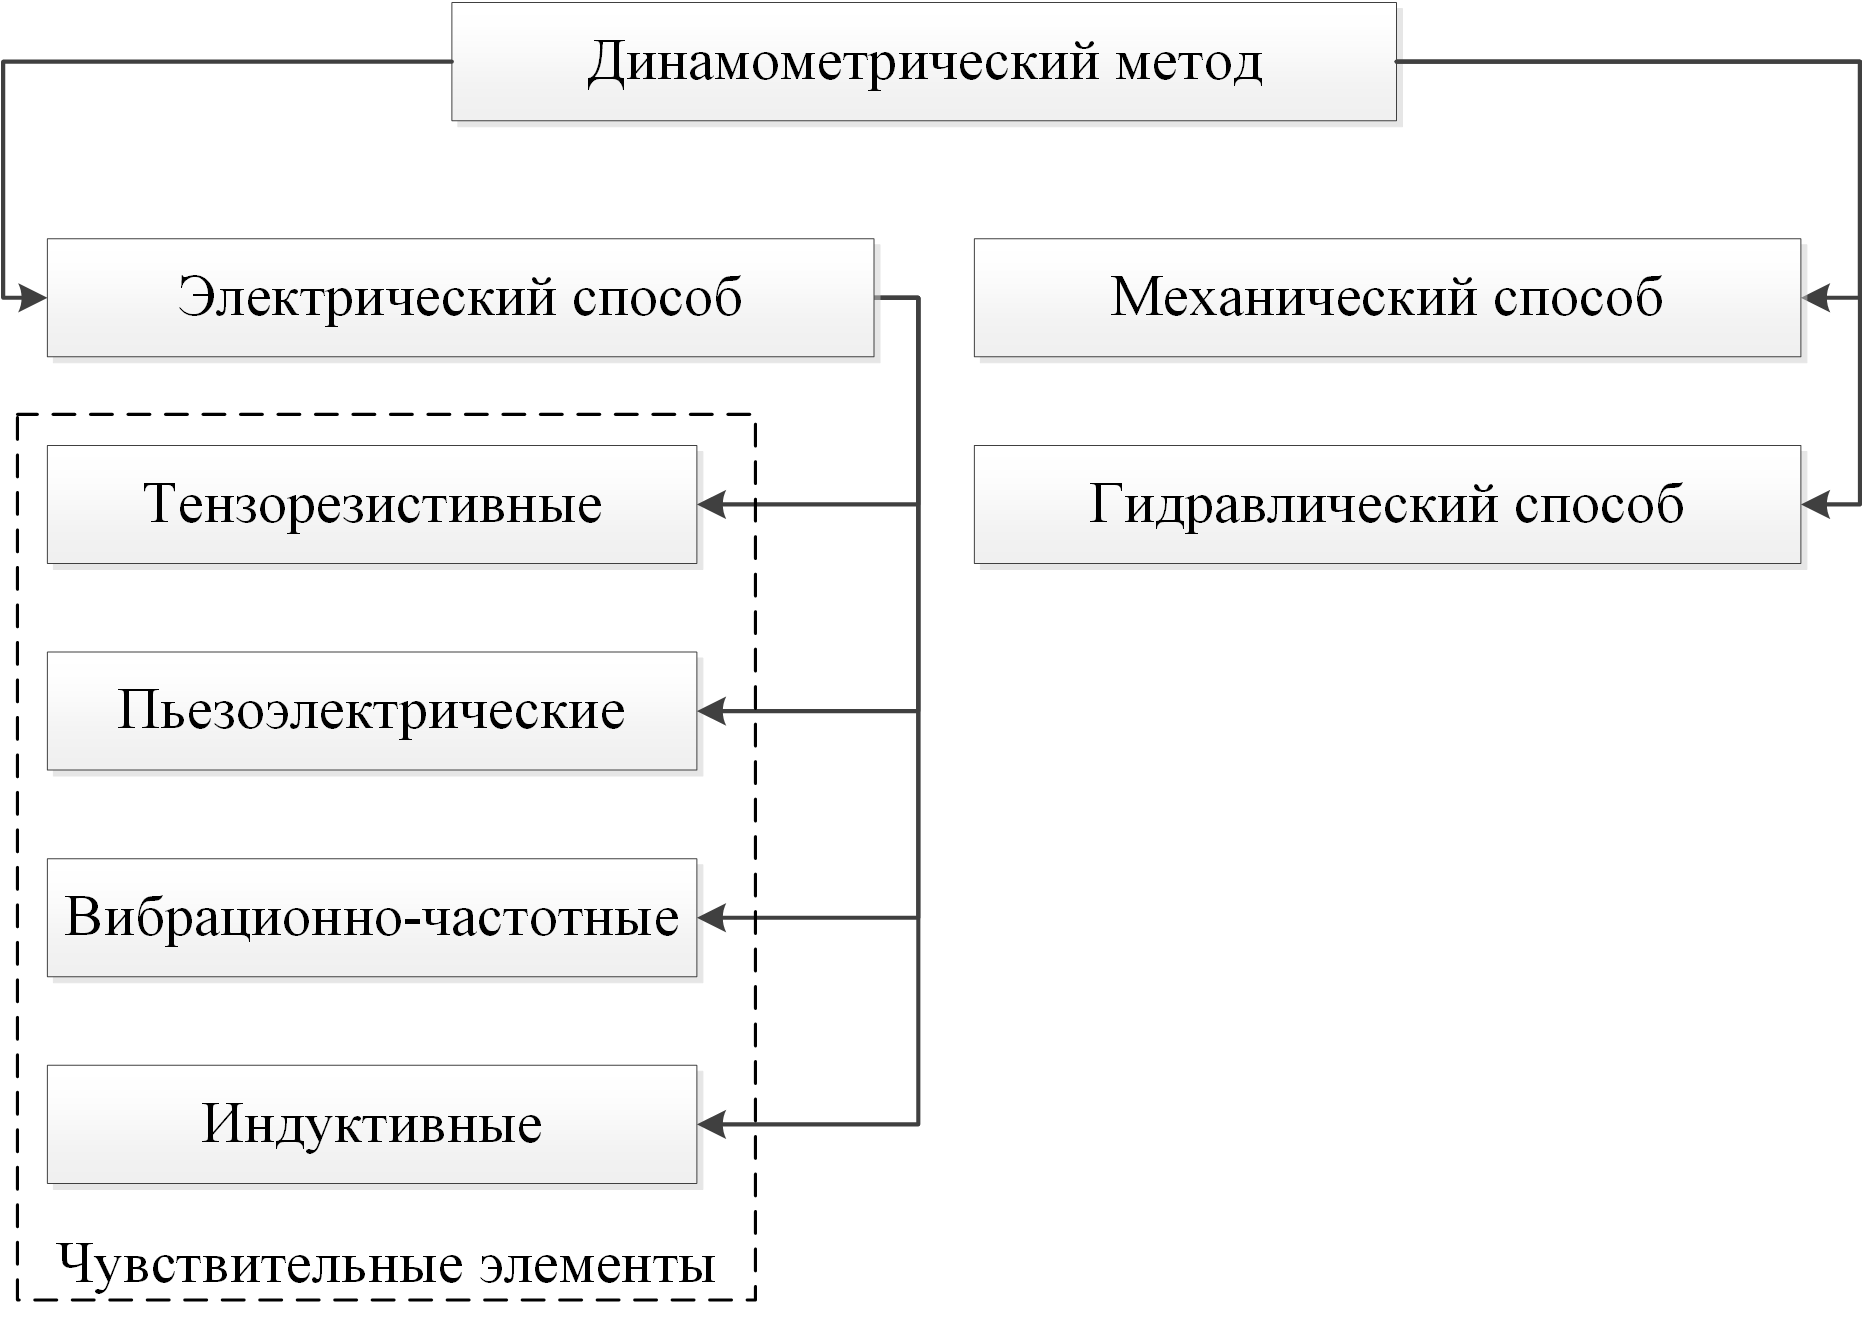
\includegraphics{MetodsControl}
	\caption{Методы контроля силовых параметров} 
	\label{img:MetodsControl}  
\end{figure}

Самым простым является механический способ так как представляет из себя прибор со шкалой либо автоматический самописец. Однако применение этого способа не целесообразно, так как имеются многочисленные недостатки, такие как: громоздкость чувствительного элемента, необходимость постоянной поверки и тарировки, не высокая точность из-за механического способа передачи информации, сложность считывания информации и т.д.

Гидравлический способ имеет в основном узко специализированное применение и не подходит для контроля силовых параметров рабочих органов из-за дороговизны и сложности конструкции.

Самым подходящим способом контроля является электрический. Он обеспечивает преобразование деформаций в электрический сигнал, который легко обрабатывать записывать и хранить. Так же одним из важнейших достоинств метода является малый размер чувствительных элементов, позволяющий устанавливать их в труднодоступных местах.

Электрический способ контроля силовых параметров обычно классифицирую в зависимости от используемых чувствительных элементов см. рисунок~\ref{img:MetodsControl}. Наиболее распространёнными являются тензорезистивные чувствительные элементы, так как:
\begin{itemize}
	\item обеспечивают достаточно высокую точность преобразования деформаций в электрический сигнал;
	\item наилучшим образом удовлетворяют критерию стоимость эффективность;
	\item могут использоваться при действии статических и динамических нагрузок;
	\item имеют линейную характеристику выходного сигнала \todo{[91]}.
\end{itemize}

\begin{table} [htbp]
	\centering
	%\captionsetup{width=17cm}
	\caption{Сравнение способов измерения усилия}
	\label{tbl:SposobIzm}
	\begin{tabular}{| l | c | c | c |}
		\hline
		\multirow{2}{*}{Критерии}&\multicolumn{3}{ c |}{Способы измерения} \\
		\cline{2-4}
		&Электрический&Механический&Гидравлический \\
		\hline
		\hline
		Стоимость				&$-$&$+$&$-$ \\
		Габаритные размеры		&$-$&$+$&$-$ \\
		Запись измерений		&$+$&$+$&$+$ \\
		Хранение измерений		&$+$&$-$&$-$ \\
		Обработка измерений		&$+$&$-$&$-$ \\
		Точность				&$+$&$-$&$+$ \\
		Сложность конструкции	&$+$&$-$&$-$ \\
		\hline
	\end{tabular}
\end{table}

\todo{Расписать то что представлено в таблицах}

\begin{table} [ht]%
	\centering
	\caption{Сравнение чувствительных элементов}%
	\label{tbl:SensItem}% label всегда желательно идти после caption
	\begin{SingleSpace}
		\setlength\extrarowheight{5pt} %вот этим управляем расстоянием между рядами, \arraystretch даёт неудачный результат
		\setlength{\tymin}{1.9cm}% минимальная ширина столбца
		\begin{tabulary}{\textwidth}{|>{\zz}L | >{\zz}C | >{\zz}C | >{\zz}C | >{\zz}C@{}|}
			\hline
			\multirow{2}{*}{Критерии}&\multicolumn{4}{ c |}{Чувствительные элементы} \\
			\cline{2-5}
			&Тензорезистивные&Пьезоэлектрические&Вибрационно-частотные&Индуктивные \\
			\hline
			\hline
			Точность преобразования	&$+$&$+$&$+$&$-$ \\
			Стоимость				&$+$&$-$&$-$&$-$ \\
			Динамические нагрузки	&$+$&$+$&$+$&$+$ \\
			Статические нагрузки	&$+$&$-$&$+$&$+$ \\
			Линейная характеристика	&$+$&$-$&$-$&$-$ \\
			Надёжность				&$+$&$-$&$-$&$-$ \\
			Доступность				&$+$&$-$&$-$&$+$ \\
			\hline
		\end{tabulary}%
	\end{SingleSpace}
\end{table}

\section{Основные выводы и задачи исследований}  \label{sect1_4}

Целью диссертационной работы является разработка метода контроля силы сопротивления прочных снежно-ледяных образований разрушению и обоснование параметров режима работы дискового режущего инструмента в зависимости от его износа.

Главными задачами проведенного комплекса научных исследований и технических разработок являются:
\begin{itemize}
	\item разработать комплекс средств контроля силы сопротивления прочных снежно-ледяных образований разрушению, возникающей в процессе взаимодействия дискового режущего инструмента с ними;
	\item исследовать влияние износа дискового режущего инструмента на силу сопротивления прочных снежно-ледяных образований разрушению;
	\item разработать математическую модель, позволяющую вычислить силу сопротивления прочных снежно-ледяных образований разрушению в зависимости от степени износа дискового режущего инструмента и шага резания;
	\item разработать метод контроля силы сопротивления прочных снежно-ледяных образований разрушению с целью минимизации энергоемкости процесса разрушения еще на стадии проектирования рабочих органов;
	\item разработать практические рекомендации по подбору радиуса закругления режущей кромки дискового режущего инструмента при проектировании рабочих органов спецмашин использующих такой инструмент.
\end{itemize}